\section{Présentation de Dynamease}

Dynamease est une start up créée par Yves Nicolas en Janvier 2014. Le modèle d'affaire de DYNAMEASE est celui d’un éditeur en mode \textit{Software As A Service} facturant à ses utilisateurs un abonnement mensuel.

\subsection{L'équipe} 

\subsubsection{Yves Nicolas}

Initiateur du projet Dynamease, son expérience multiple et sa polyvalence sur les sujets techniques, marketing et commerciaux lui ont permis de créer l’entreprise Dynamease, en ayant la vision stratégique, marketing et la mise en œuvre technologique de l’entreprise. Il était mon maître de stage et mon chef de projet.

\subsubsection{Etienne Laplane}

Employé de Dynamease en charge de l’architecture du service Dynamease et du serveur pour les communications téléphoniques : Asterisk.


\section{Présentation du service Dynamease}

\subsection{Les objectifs}

Dynamease se base sur le fait que le portable devient l'appareil de communication majoritaire par rapport aux téléphones fixes. Le portable devient, grâce à Dynamease, un standard automatisé. Tous les appels entrant sont filtrer en amont afin de déterminer leur importance et leur provenance. Il est possible pour un client Dynamease de configurer les services Dynamease afin de déterminer les horaires d'appel pour différent type de contact (Professionnel, Familial, amis).

Une fois les appels filtrés, ils sont redirigés vers l'appareil téléphonique indiqué par l'utilisateur.

Les appels sont ensuite redirigés des informations récupérées sur les bases de données privées du clients ainsi que sur des bases de données publique (Annuaire inverse, réseaux sociaux ...) sont affichées sur l'appareil téléphonique du client.\\

Ce service permet au client de déléguer la partie standardisation de son entreprise et de ne plus rater des appels important tout en ignorant les appels nuisibles. De plus Dynamease propose aux entreprises de diminuer leurs coûts de téléphonie en remplaçant les appareils fixes de l'entreprise par les téléphones portable des employés. Les employés pourront ainsi avoir un seul appareil téléphonique pour leur appel, et configurer leurs horaires d'appel en fonction de leurs horaires de travail pour en pas être dérangé.

\subsection{Les différentes offres}

Dynamease propose à ses clients plusieurs offres. Chaque offre contient des fonctionnalités particulières. Chaque offre contient les fonctionnalités des offres qui la précédent dans la hiérarchie. La hiérarchie des offres Dynamease est la suivante :

\begin{figure}[!h]
	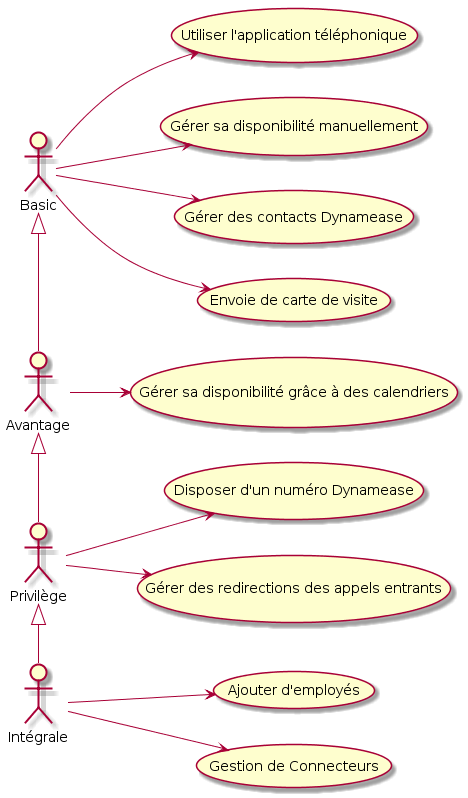
\includegraphics[scale=0.5]{img/useCase.png}
	\caption{\label{useCase} Diagramme de cas d'utilisation Dynamease}
\end{figure}

Nous allons maintenant décrire les différentes offres.

\subsubsection{Basic}

L'offre Basic est une offre gratuite, elle permet à l'utilisateur d'accéder aux fonctions basiques de l'application téléphonique et de l'application web:

\begin{itemize}
	\item Envoie de carte de visite Dynamease;
	\item Gestion de la liste de contact;
	\item Gestion manuelle de la disponibilité.
\end{itemize}

\subsubsection{Avantage}

L'offre Avantage s'adresse aux particuliers, désirant avoir une gestion de sa disponibilité gérer par rapport à des calendrier (Calendrier Dynamease ou \textit{Google Calendar}).

\subsubsection{Privilège}

L'offre Privilège permet aux utilisateurs d'obtenir un numéro Dynamease. Ce numéro permet à l'utilisateur d'être joint sur un de ses appareils téléphoniques selon les choix de l'utilisateur. Les appels entrant en direction du numéro Dynamease sont gérés par le serveur Dynamease. Celui-ci identifiera l'appel, définira sont importance et enfin le redirigera vers l'appareil défini par l'utilisateur.

\subsubsection{Intégrale}

L'offre Intégrale est destinée pour les entreprises. Cette offre permet l'ajout d'employé qui auront les mêmes fonctionnalité qu'un compte Avantage.

Il est également possible d'ajouter des connecteurs. Les connecteurs permettent une meilleure identification d'appel ainsi qu'une meilleure redirection. Les connecteurs sont des données fournies par les entreprises qui permettent d'identifier leurs clients ainsi que l'employé responsable du client identifié. Les connecteurs sont donc utilisés pour fournir des informations sur l'appelant et également sur la redirection de l'appel.

\section{Présentation de l'environnement Dynamease}

\subsection{Environnement du service Dynamease}

Nous allons maintenant présenter l'environnement Dynamease. Dynamease suit le pattern MVC (Modèle View Controler). On peut représenter l'environnement principal de Dynamease avec le diagramme suivant.

[Mettre diagramme]

Présentons ce diagramme du haut vers le bas. Nous avons en haut les application utilisant les service Dynamease. Ces applications sont la partie web, accessible pour l'utilisateur depuis un navigateur et les applications téléphoniques constituées par les applications Android et Ios.

Pour utiliser les services Dynamease sont accessible via les interfaces de requêtes représenté par JsonRq et Appless. JsonRq réuni toutes les requêtes de type json RPC et Appless réuni toutes les requêtes REST. Dynamease dispose de ces deux interfaces car une migration est entrain d'être effectuée, toutes les requêtes deviendront des requêtes de type Json RPC.

En ce qui concerne la partie Controler, Dynamease dispose de trois partie. La première partie représenté par le Matcher, représente la recherche du contact lors d'un appel. La partie classif réunie toutes les classes aidant à la classification de l'appelant. Et enfin la partie infoBuilder, construit les informations relatives à l'appelant afin de les fournir à la personne recevant l'appel.

La partie Modèle de Dynamease est représentée par les parties Core et Kernel. Core représente les classes métier utilisé uniquement par le serveur Dynamease. Quant à la partie Kernel elle réunie toutes les classes pouvant être utilisées par chacune des applications de Dynamease.

Le stockage est géré par deux bases de données Mysql et Ldap. La base de données Ldap est utilisé pour stocker les informations sur les contacts des utilisateurs. La base MySQL stocke toutes les autres informations utiles.

La raison de la présence de deux base de données et du au fait de répondre à un besoin des futurs clients ayant déjà un annuaire Ldap, afin de faciliter l'importation de ces contacts.\\\\

en plus du serveur Dynamease, l'entreprise dispose aussi d'un serveur Asterisk. C'est un serveur gérant les communications téléphoniques. Ce serveur communique avec le serveur Dynamease afin de gérer les redirections et avoir les numéros entrant.\\

Un serveur Aerogear est également mis en place pour la gestion des notifications Push. Une présentation détaillée de ce serveur sera effectuée dans la suite de ce rapport.